

\section{Overall Description}
This section provides an overview of the requirements and specifications for the e-commerce application for a sports equipment shop. The application will manage products, orders, and payments. Inventory management will not be included in the initial version of the system but is planned for a future update.
\subsection{Product Perspective}
The e-commerce application is intended to provide a user-friendly, scalable, and reliable online platform for a sports equipment shop. It aims to overcome the limitations of traditional monolithic architecture and effectively manage the fundamental requirements of an e-commerce website.
\subsection{Product Functions}
The e-commerce application will include the following functions:
\begin{itemize}
    \item[-] \textbf{User Authentication:} Allows users to register and log in to their accounts.
    \item[-] \textbf{Product Management:} Enables administrators to manage the type, brand and products available on the website.
    \item[-] \textbf{Order Management:} Enables administrators to manage orders and update the order status on the website.
    \item[-] \textbf{Order Processing:} Handles the processing of customer orders.
    \item[-] \textbf{Payment Processing:} Manages the payments for customer orders.
    \item[-] \textbf{Product Browsing:} Provide user to view or search list of products available on the store.
          \begin{itemize}
              \item Search by filter and sort: Allows users to search for products available on the platform.
              \item Product views: Provides detailed information about a product or products by type or brand.
          \end{itemize}
    \item[-] \textbf{Wishlist: } Allows users to save their favorite products for later viewing.
    \item[-] \textbf{Basket: } This function allows users to add products to their shopping basket. The Basket page displays a list of products in the user's shopping basket, allowing them to view, update quantities, and remove items. Users can proceed to checkout to complete the purchase.
    \item[-] \textbf{Order: } This function allows users to track the order status of their order and other informations of order.
\end{itemize}
\subsection{User Classes and Characteristics}
The application will have two main types of users: customers who are looking to purchase sports equipment, and administrators who manage the products, orders, and payments.
\subsection{Operating Environment}
The application will be developed using the MEVN stack (MongoDB, Express.js, Vue.js, Node.js) and will be designed to operate on various platforms and devices.

\section{ Requirements Specification}
\subsection{ External Interface Requirements}

The application will have a user-friendly interface for customers to browse products, place orders, and make payments. It will also have an administrative interface for managing products, orders, and payments.

\subsection{ Functional Requirements}
\subsubsection{User Use Cases}
\begin{figure}[H]
    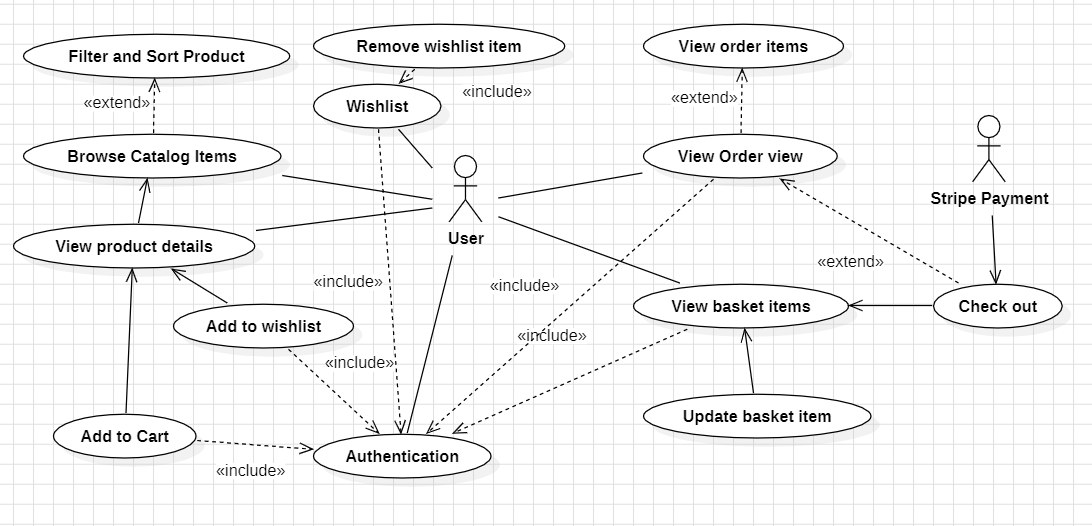
\includegraphics[width=\linewidth]{User-Actor.png}
    \caption{User usecase}
    \label{fig:admin-user-usercase}
\end{figure}
\begin{enumerate}
    \item \textbf{User Authentication:} The user registers and logs in to their account. This is the first step for users to interact with the system.
    \item \textbf{Product Browsing:} The user views or searches the list of products available on the store. This includes searching for products by filter and sort, and viewing detailed information about a product or products by type or brand.
    \item \textbf{Wishlist:} The user saves their favorite products for later viewing. This allows users to keep track of items they are interested in but are not ready to purchase yet.
    \item \textbf{Basket:} The user adds products to their shopping basket, views, updates quantities, and removes items. The user proceeds to checkout to complete the purchase. This is the main function for users to purchase products.
    \item \textbf{Order:} The user tracks the order status of their order and other information of the order. This allows users to keep track of their purchases and expected delivery times.
\end{enumerate}
\subsubsection{Admin Use Cases}
\begin{figure}[H]
    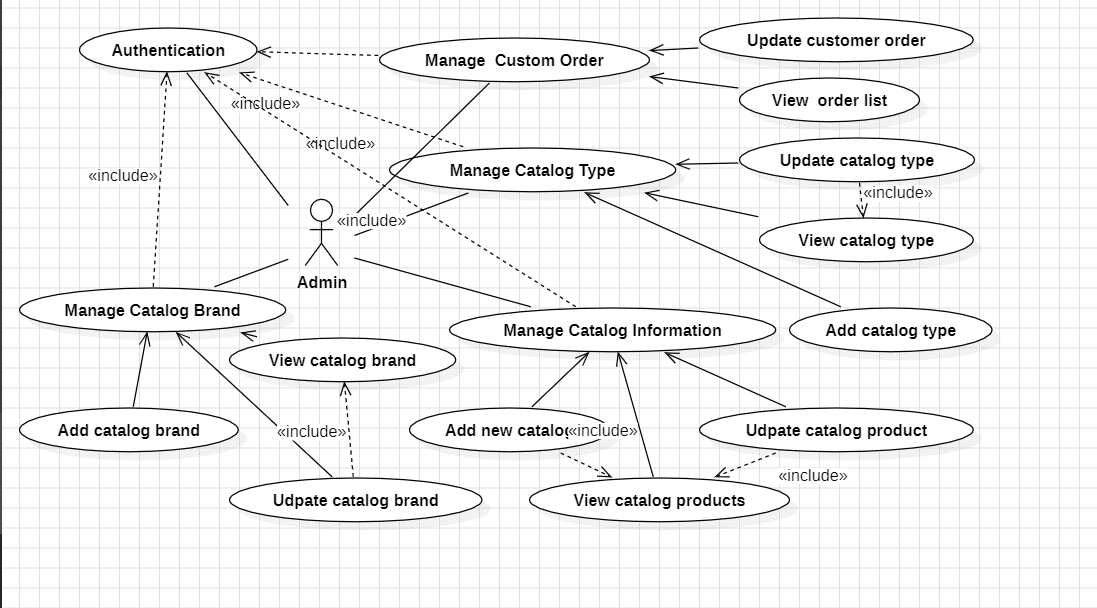
\includegraphics[width=\linewidth]{Admin-Actor.png}
    \caption{Admin usecase}
    \label{fig:admin-admin-usecase}
\end{figure}
\begin{enumerate}
    \item \textbf{Product Management:} The administrator manages the type, brand, and products available on the website. This is crucial for keeping the product catalog up to date and relevant to the customers.
    \item \textbf{Order Management:} The administrator manages orders and updates the order status on the website. This is important for ensuring that orders are processed and delivered in a timely manner.
\end{enumerate}
\subsection{ Nonfunctional Requirements}
The application will be designed to be scalable, allowing it to handle a growing number of products and users. It will also be reliable, ensuring that it operates correctly and provides accurate information.

Each function and requirement will be described in detail, including its purpose, how it works, and how it contributes to the overall functionality of the e-commerce application.